\documentclass[11pt,a4paper]{article}
\usepackage{moesio}
\usepackage{caption}
\pgfplotsset{compat=1.18}
%==========================================================================================
\newcommand{\nomet}{\bf Msc. Moésio}
\newcommand{\nome}{\bf Moésio M. de Sales}
\newcommand{\nomer}{Matemática Discreta}
\newcommand{\titu}{Avaliação $N1$ -- $4.5$ Pontos}
\newcommand{\disc}{Matemática Discreta}
\newcommand{\curso}{Sistemas de Informação}
\newcommand{\inst}{IFCE}
%==========================================================================================
\begin{document}
\Large
\begin{center} \titu\\ \disc\\ \curso\\  \nome\footnote{moesio@ifce.edu.br} \end{center}
%==========================================================================================
\framebox[8.6\width]{Alun@:\hfill}\fbox{\today}\\
%==========================================================================================
\fbox{\begin{minipage}{35.4em}
  Respostas sem justificativas não serão consideradas na correção.
\end{minipage}
}

\bexer
%=========================================================================
\item 
 Seja $A = \{1, 2, 3, 4, 8\}$ e $B = \{1, 2, 3, 4\}$ e defina as relações binárias $R$ e $S$ como:
 \ben
\forall (x, y)\ \in\ A \times B,\ xRy\ \Leftrightarrow\ x^2 -y^2=x+y, \\
\forall (x, y)\ \in\ A \times B,\ xSy\ \Leftrightarrow\  \frac{x}{y} \in B.
\een
\begin{enumerate}
\item Liste os pares ordenados que estão em:
\begin{enumerate}
	\item $R$; 
	\item $S$; 
\end{enumerate}
\item $R\circ S$;
\item $S\circ R$ 
\end{enumerate}



\item Mostre se a relação binária
$P$ é reflexiva, simétrica, transitiva. Seja a relação $P$ definida sobre
$\mathbb{R}-\{0\}$ como:
\ben x, y\in \mathbb{R},\ xPy\ \Leftrightarrow\ xy> 0 \een


        	
\item Seja $A=\mathbb{R}$. Para $a, b\in A^\ast=A-\{0\}$, definimos
\[ aRb  \Leftrightarrow ab =x^2+y^2
,\]
para alguns $x$, $y\in A$. Mostrar que é uma relação de equivalência em $A^\ast$.


\item
  Seja $A =\{2,3,4,5,6,7,8,9\}$  a relação binária $R$ em $A$ definida como
  \[ \forall (x,y) \in A\times A,\ xRy\ \Leftrightarrow\ x|(x-y)\]
  \begin{enumerate}
	\item Liste os pares de $R$;
	 \item Desenhe o grafo de $R$;
	\item  Determine se a relação é: reflexiva; simétrica; transitiva.
	  \item Se $R$ for relação de equivalência, determine $A/R$.
	  \end{enumerate}


\item  Considere a relação $R$ sobre  $A=\{2,4,5,6,7,8\}$
 \[  aRb\ \Leftrightarrow\  mdc(a; b) = 1\]
 Verifique se $R$ é:
\begin{multicols}{3}
\begin{enumerate}
\item Reflexiva
\item Simetrica
\item Transitiva
\end{enumerate} 
\end{multicols}
  
\item
  Seja $A =\{2,3,4,6,7,9\}$  a relação binária $R$ em $A$ definida como
  \[ \forall (x,y) \in A\times A,\ xRy\ \Leftrightarrow\ 3|(x-y)\]
  \begin{enumerate}
	\item Liste os pares de $R$;
	\item  Determine se a relação é: reflexiva; simétrica; transitiva.
	  \item Se $R$ for relação de equivalência, determine $A/R$.
	  \end{enumerate}



\item Verifque se a relação $S$ dada por
\[S = \{(x,y)\in \mathbb{Z}\times \mathbb{Z};|x-y|\leq 4\}\]
é:
		\begin{enumerate}
				\item Reflexiva.
				\item Simétrica.
				\item Tansitiva.
		\end{enumerate}

 
\item
  Seja $S =\mathbb{N}$ e seja uma relação binária em $S$ definida por
  \[
	xRy \Leftrightarrow x^2-y^2\ \text{é par}
  \]
  \begin{enumerate}
	\item 	Mostre que $R$ é uma relação de equivalência em $S$;
	\item Descreva as classes de equivalência que define $R$.
  \end{enumerate}

\item 
 Seja $A = \{1,2,3,4,5\}$ e $B = \{5,6,8,9,10\}$ e defina as relações binárias $R$ e $S$ como:
 \ben
\forall (x, y)\ \in\ A \times B,\ xRy\ \Leftrightarrow\ (x-2)^2|y, \\
\forall (x, y)\ \in\ A \times B,\ xSy\ \Leftrightarrow\  y +1 = x^2.
\een
Liste os pares ordenados que estão em:
\begin{enumerate}
\item $R$;
\item $S$;
\item $R \circ S$;
\item Faça um esboço do grafo de $R$;
\item Considere que $S$ é uma relação de $A$ em $A$, escreva a matriz da relação $S$;
\item Considere que $R$ é uma relação de $A$ em $A$, escreva a matriz da relação $R$;
\end{enumerate}


\item Dada a matriz $M=(m_{ij})$
\[ 
M=\begin{bmatrix}
1&0&1&1 \\0&1&0&1 \\1&0&1&1 \\ 1&1&1&1
\end{bmatrix}
\]
e o conjunto $A=\{a_1,a_2,a_3,a_4\}$, defini-se em $A$ uma relação $R$ dada por:
\[
a_iRa_j\ \Leftrightarrow\   m_{ij}=1
\] 
\begin{enumerate}
  \item Verifique se a relação $R$ é de equialência.
  \item Determine $A/R$.
\end{enumerate}

\begin{minipage}[bt]{0.5\linewidth}
%==============================================================
\item Seja $A = \{a, b, c, d, e, f\}$ o conjunto das retas da figura ao lado :
Para a relação 
\[
xRy\ \Leftrightarrow\ x\  \mbox{é paralela a}\ y
\]
Mostre que $R$ é uma relação de equivalência.
%==============================================================
\end{minipage}
%==============================================================
\hspace{0.04\textwidth}
%==============================================================
\begin{minipage}[h]{0.4\linewidth}
\centering
%==============================================================
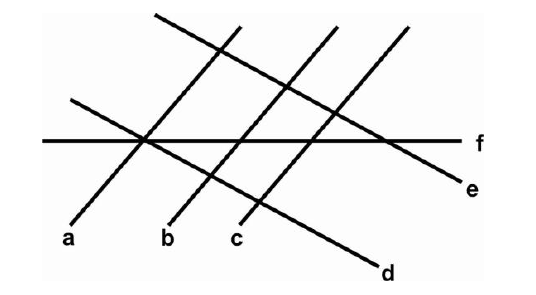
\includegraphics[scale=.5]{fig1-q49.png}
%==============================================================
%\caption{Histograma Exemplo~\ref{exe1-moda}} %
\end{minipage}
%\end{figure}
  
\item Sejam $P$ e $R$ relações binárias em $\mathbb{N}$ definidas por
  \[\
	xPy \Leftrightarrow ''x\ \text{divide}\ y''\ \text{e}\ \ xRy\ \Leftrightarrow\ 5x\leq y. 
  \]
Determine quais dos pares ordenados satisfazem às relações dadas:
\begin{enumerate}
  \item $P\cup R:(2,6),(3,17),(2,1),(0,0)$
  \item $P\cap R:(3,6),(1,2),(2,12)$ 
  \item $\overline{P}:(1,5),(2,8),(3,15)$ 
  \item $\overline{R}:(1,1),(2,10),(4,8)$ 
\end{enumerate}

\item
 Sejam $E = \{x \in \mathbb{Z}| - 7 \leqslant x \leqslant 7\}$ e $R$ a relação sobre $E$ definida por
 \ben
xRy\ \Leftrightarrow\ x^2 + 2x = y^2 + 2y.
\een
\begin{enumerate}
\item  $R$ é  reflexivo? (Justifique) 
\item  $R$ é  simétrico? (Justifique) 
\item  $R$ é  transitivo? (Justifique) 
\item  $R$ é relação de equivalência? (Justifique)
\item Descreva as classes de equivalência $\overline{0}$,$\overline{-2}$ e $\overline{4} $.
\end{enumerate}

\item Seja a relação $P$ definida sobre
$\mathbb{R}$ como:
\ben x, y\in \mathbb{R},\ xPy\ \Leftrightarrow\ xy\geqslant 0 \een

\begin{enumerate}
\item A relação $P$ é reflexiva? Simétrica? Justifique.
\item A relação $P$ é transitiva? Justifique.
\end{enumerate}


\item %pag 170
		Seja $A=\{1,2,3,4\}$ e $R$ uma relação em $A$ definida por
\[ 
M=\begin{bmatrix}
1 & 0 & 0 & 0 \\
0 & 1 & 1 & 1 \\
0 & 1 & 1 & 1 \\
0 & 1 & 1 & 1 
\end{bmatrix}
\]
Determine $A/R$.

\item 
		Seja $R$ uma relação de equivalência em um conjunto onde a operação $+$ é difinida como {\sc Soma de R-relativos}, como segue:
		\[
				R(a) + R(b) = \{x|\ x=s+t,\ s\in R(a)\ \text{e}\ t\in R(b)\}
		\]
Dada a relação definida por:
\[R=\{(a,b)\in \mathbb{N}\times \mathbb{N}|\ a\equiv b (mod\ m) \]
Mostre que $R(a)+R(b)=R(a+b),\ \forall a,b$				

\item 
		Sejam $A=\{1,2,3,4,5\}$ e $M_R$ e $M_s$ matrizes das relações $R$ e $S$ em $A$.
\[ 
M_R=\begin{bmatrix}
1 & 0 & 1 & 1 & 1\\
0 & 1 & 1 & 0 & 0\\
1 & 0 & 0 & 1 & 0\\
1 & 0 & 1 & 0 & 0\\
0 & 1 & 1 & 1 & 1
\end{bmatrix}
\
M_S=\begin{bmatrix}
1 & 0 & 1 & 1 & 1\\
0 & 1 & 1 & 0 & 0\\
1 & 0 & 0 & 1 & 0\\
1 & 0 & 1 & 0 & 0\\
0 & 1 & 1 & 1 & 1
\end{bmatrix}
\]
Determine:
\begin{multicols}{2}  
\begin{enumerate}
		\item $M_{R\circ R}$
		\item $M_{S\circ S}$
		\item O fecho transitivo de ${R\cap S}$.
		\item O fecho transitivo de $(R\cup S)$
\end{enumerate}
\end{multicols}

\item 
		Sejam $A=\{a_1,a_2,a_3,a_4,a_5\}$ e $R$ uma relação  em $A$, dada por 
\[ 
M_R=\begin{bmatrix}
1 & 0 & 1 & 1 & 1\\
0 & 1 & 1 & 0 & 0\\
1 & 0 & 0 & 1 & 0\\
1 & 0 & 1 & 0 & 0\\
0 & 1 & 1 & 1 & 1
\end{bmatrix}
\]
\begin{enumerate}
		\item Determine $W_3$
		\item Determine $R^{\infty}$ pelo algorítmo de Warshall.
\end{enumerate}

\eexer
%=========================================================================
\end{document}
